%% Springer Nature LaTeX template, npj Microgravity style (sn-jnl.cls and sn-nature.bst copied,
%% already patched, from the first study's manuscript; see README.md).
\documentclass[pdflatex,sn-nature]{sn-jnl}

\usepackage{graphicx}
\usepackage{amsmath,amssymb,amsfonts}
\usepackage{booktabs}
\usepackage{tabularx}
\newcolumntype{L}{>{\raggedright\arraybackslash}X}
\usepackage{textcomp}
\usepackage{url}

\graphicspath{{../../results/figures/}}
% Generated by scripts/18_manuscript_numbers.py. Do not edit by hand.
\newcommand{\nSourceRows}{161}  % T01
\newcommand{\nSourceKegg}{123}  % T01
\newcommand{\nZhuAcc}{259}  % T01
\newcommand{\nWuAcc}{301}  % T01
\newcommand{\nCaldanaMin}{14}  % T01
\newcommand{\nCaldanaMax}{18}  % T01
\newcommand{\nRefCompounds}{96}  % T02
\newcommand{\nRefRobust}{45}  % T02
\newcommand{\nRefSingle}{22}  % T02
\newcommand{\nRefNone}{28}  % T02
\newcommand{\nRefConflicting}{1}  % T02
\newcommand{\nRefUp}{24}  % T02
\newcommand{\nRefDown}{43}  % T02
\newcommand{\leuZhu}{4.92}  % T01
\newcommand{\leuWu}{4.74}  % T01
\newcommand{\leuCaldana}{2.40}  % T01
\newcommand{\ileZhu}{3.15}  % T01
\newcommand{\ileWu}{4.42}  % T01
\newcommand{\gluWu}{-0.50}  % T01
\newcommand{\gluWuFrac}{97}  % T01
\newcommand{\glnWu}{-0.02}  % T01
\newcommand{\glnWuFrac}{50}  % T01
\newcommand{\serZhu}{-0.29}  % T01
\newcommand{\serZhuFrac}{83}  % T01
\newcommand{\malZhu}{-1.19}  % T01
\newcommand{\oxgZhu}{-1.68}  % T01
\newcommand{\asnCaldana}{1.51}  % T01
\newcommand{\ratioLeuVal}{2.8}  % T02
\newcommand{\ratioLeuAsn}{2.7}  % T02
\newcommand{\nModelCompounds}{21}  % first study T06
\newcommand{\nComparable}{6}  % T03
\newcommand{\nScored}{12}  % T03
\newcommand{\nModelAgree}{5}  % T03
\newcommand{\nModelDisagree}{1}  % T03
\newcommand{\nModelUntested}{6}  % T03
\newcommand{\nModelNotComparable}{9}  % T03
\newcommand{\nNotPredicted}{59}  % T03
\newcommand{\nNotPredictedRobust}{41}  % T03
\newcommand{\nTests}{36}  % T08
\newcommand{\nMatch}{18}  % T08
\newcommand{\nLitMatch}{5}  % T08
\newcommand{\nDarkMatch}{13}  % T08
\newcommand{\nLitTests}{18}  % T08
\newcommand{\nSigLitPredicted}{0}  % T08
\newcommand{\pDinFiveTwoTwo}{= 0.0281}  % T08
\newcommand{\qDinFiveTwoTwo}{= 0.127}  % T08
\newcommand{\zDinFiveTwoTwo}{2.4}  % T08
\newcommand{\pDinLight}{= 0.089}  % T08
\newcommand{\qDinLight}{= 0.229}  % T08
\newcommand{\zDinLight}{1.7}  % T08
\newcommand{\pDinFourTwoSeven}{= 0.0318}  % T08
\newcommand{\qDinFourTwoSeven}{= 0.127}  % T08
\newcommand{\zDinFourTwoSeven}{2.2}  % T08
\newcommand{\pBcaaLight}{= 0.0397}  % T08
\newcommand{\qBcaaLight}{= 0.143}  % T08
\newcommand{\zBcaaLight}{2.0}  % T08
\newcommand{\pDinThirtyEight}{= 0.0015}  % T08
\newcommand{\qDinThirtyEight}{= 0.0108}  % T08
\newcommand{\zDinThirtyEight}{-3.4}  % T08
\newcommand{\pDinThreeTwoOne}{\le 10^{-4}}  % T08
\newcommand{\qDinThreeTwoOne}{= 0.0018}  % T08
\newcommand{\zDinThreeTwoOne}{-5.6}  % T08
\newcommand{\pDinDark}{= 4.00\times10^{-4}}  % T08
\newcommand{\qDinDark}{= 0.0048}  % T08
\newcommand{\zDinDark}{3.9}  % T08
\newcommand{\pBcaaThreeTwoOne}{\le 10^{-4}}  % T08
\newcommand{\qBcaaThreeTwoOne}{= 0.0018}  % T08
\newcommand{\zBcaaThreeTwoOne}{-6.9}  % T08
\newcommand{\pBcaaDark}{= 1.00\times10^{-3}}  % T08
\newcommand{\qBcaaDark}{= 0.009}  % T08
\newcommand{\zBcaaDark}{3.4}  % T08
\newcommand{\pSharedLight}{= 0.0019}  % T08
\newcommand{\qSharedLight}{= 0.0114}  % T08
\newcommand{\zSharedLight}{2.8}  % T08
\newcommand{\pDarkMetFiveTwoTwo}{= 0.0281}  % T08
\newcommand{\qDarkMetFiveTwoTwo}{= 0.127}  % T08
\newcommand{\zDarkMetFiveTwoTwo}{2.1}  % T08
\newcommand{\pDinFiveTwoTwoMW}{= 0.0026}  % T08
\newcommand{\pDinFiveTwoTwoRot}{= 0.0087}  % T08
\newcommand{\pDinFirstStudy}{= 0.0026}  % first study T07
\newcommand{\nSetDin}{5}  % prereg/gene_sets.tsv
\newcommand{\nSetBcaa}{53}  % prereg/gene_sets.tsv
\newcommand{\nSetWuControl}{301}  % prereg/gene_sets.tsv
\newcommand{\nSetWuStress}{491}  % prereg/gene_sets.tsv
\newcommand{\nSetWuShared}{1{,}954}  % prereg/gene_sets.tsv
\newcommand{\nSetWuDarkMet}{540}  % prereg/gene_sets.tsv
\newcommand{\nPathOne}{6}  % T07
\newcommand{\nHubOne}{7}  % T07
\newcommand{\nHubTestedOne}{15}  % T07
\newcommand{\nPathA}{6}  % T07
\newcommand{\nHubA}{11}  % T07
\newcommand{\nHubTestedA}{32}  % T07
\newcommand{\nPathB}{24}  % T07
\newcommand{\nHubB}{17}  % T07
\newcommand{\nHubTestedB}{32}  % T07
\newcommand{\nPathC}{10}  % T07
\newcommand{\nHubC}{5}  % T07
\newcommand{\nHubTestedC}{32}  % T07
\newcommand{\rhoOneA}{0.95}  % T04
\newcommand{\rhoBC}{0.51}  % T04
\newcommand{\nPathTotal}{232}  % T04
\newcommand{\rankGlyOne}{214}  % T04
\newcommand{\rankGlyA}{193}  % T04
\newcommand{\pPhotoC}{= 1.03\times10^{-12}}  % T04
\newcommand{\qPhotoB}{= 0.131}  % T04
\newcommand{\pBcaaDegC}{= 0.00506}  % T04
\newcommand{\pBcaaDegB}{= 0.0854}  % T04
\newcommand{\pErA}{= 8.65\times10^{-9}}  % T04
\newcommand{\hubLightFDR}{0.044}  % T05
\newcommand{\nSharedHubSteps}{16}  % T07
\newcommand{\nLayer}{96}  % data/paintomics_upload/metabolomics_key.tsv
\newcommand{\nLayerRelevant}{45}  % data/paintomics_upload/metabolomics_key.tsv
\newcommand{\nDELight}{7{,}790}  % data/osdr/contrast_OSD-678-light
\newcommand{\nDEDark}{2{,}112}  % data/osdr/contrast_OSD-678-dark
\newcommand{\ratioDE}{3.7}  % data/osdr
\newcommand{\nPanel}{29}  % T10
\newcommand{\nPanelGroups}{19}  % data/reference/metabolights_group_sds.tsv
\newcommand{\nPanelStudies}{6}  % data/reference/metabolights_group_sds.tsv
\newcommand{\sdMin}{0.31}  % T10
\newcommand{\sdMax}{1.21}  % T10
\newcommand{\nQThousandMin}{92}  % T10
\newcommand{\nQThousandMax}{1{,}342}  % T10
\newcommand{\nQSixtyMin}{1{,}293}  % T10
\newcommand{\detectMin}{0.56}  % T10
\newcommand{\detectMinFold}{1.48}  % T10
\newcommand{\nTwoFoldMax}{24}  % T10
\newcommand{\qSixtyLogTwo}{0.035}  % first study T13


\begin{document}

\title[Light/dark metabolism tests a spaceflight carbon-starvation model]{Natural variation in
\textit{Arabidopsis} light/dark metabolism tests a carbon-starvation model of plant spaceflight
transcriptomes}

%% TODO AUTHORSHIP --- every field below except the corresponding author is a placeholder,
%% as in the first study's manuscript. See README.md for the checklist.
\author*[1]{\fnm{Richard} \sur{Barker}}\email{dr.richard.barker@gmail.com}
\affil[1]{\orgname{[TODO --- affiliation]}, \city{[TODO]}, \country{[TODO]}}

\abstract{A gas-transport and photosynthesis model of the BRIC-LED-001 flight (OSD-522) predicted
that microgravity lowers net assimilation whenever plants are lit, so that lit spaceflight
transcriptomes should carry a carbon-starvation signature and dark ones should not. It also
predicted metabolite shifts that could not be checked, because NASA's Open Science Data Repository
holds no plant metabolome. Here we test that model against measured extended-darkness metabolism,
used as a direction-of-change reference for carbon limitation: leaf metabolomes of \nZhuAcc{}
accessions before and after six days of darkness, \nWuAcc{} accessions under control conditions
and darkness at 32\,\textdegree C with their metabolite GWAS loci, and a light/dark time course.
Darkness raised leucine and isoleucine in every accession of both natural-variation panels, under
every qualification threshold we tried. Darkness can test only \nScored{} of the model's
\nModelCompounds{} compound predictions, and \nComparable{} of those have a measured direction;
\nModelAgree{} agreed. The one disagreement, a fall in glutamate, rests on the 32\,\textdegree C
source alone, and \nNotPredictedRobust{} robust darkness responses, among them TCA-cycle acids and
flavin and nicotinamide cofactors, were not predicted. In PaintOmics, replacing the model's
metabolite layer with \nLayer{} measured compounds, removing it, or rescaling its values left the
pathway result unchanged; hub calls needed the gene and protein layers together and disappeared when
the light contrast's differentially expressed genes were cut to the dark contrast's number. Of
\nTests{} pre-registered gene-set outcomes, \nMatch{} matched. No predicted lit-flight starvation
signal reached significance, while carbon-starvation and branched-chain amino acid catabolism genes
moved strongly in three dark flight contrasts, down in two BRIC canister experiments and up in the
leaves of dark-grown CARA seedlings; these calls rest on a gene-level null that we show to be
calibrated, because three plants per arm leave sample permutation too coarse to confirm them. In
OSD-38, a dark sealed-BRIC flight with a proteome, the four KEGG carbon pathways rose in the
transcriptome but fell in the membrane fraction of the proteome, and on the ground the BRIC-PDFU
carried a strong low-oxygen transcript signature against an air-tight container. With six plants
per arm a targeted GC-MS panel could detect only changes of about \detectMinFold-fold or larger;
the model's predicted 0.13\,log$_2$ shifts would need \nQThousandMin{} to \nQThousandMax{} plants
per arm. The carbon-starvation signal in plant spaceflight transcriptomes is real, but it is not
specific to light, its sign differs between flight experiments, and where proteins were measured,
carbon metabolism moved against its transcripts.}

\keywords{spaceflight, \textit{Arabidopsis}, natural variation, carbon starvation, darkness,
metabolomics, proteomics, pre-registration}

\maketitle

\section{Introduction}\label{sec:intro}

A companion study \citep{firststudy} coupled a lattice-Boltzmann model of leaf boundary-layer gas
transport to a Farquhar--von Caemmerer--Berry model of photosynthesis and asked what the sealed,
illuminated BRIC-LED canister of OSD-522 \citep{osd522} does to the CO$_2$ reaching Rubisco. It
predicted that microgravity, by suppressing buoyant convection, leaves a persistent deficit in net
assimilation whenever the plants photosynthesise, and that the flight transcriptome should
therefore show a mild carbon-starvation response. Because there is no assimilation to lose in the
dark, the same model predicts no such response in dark-grown flight experiments.

That study left four things open. Its metabolite predictions could not be tested, because the NASA
Open Science Data Repository \citep{osdr2025} contains no plant metabolome; it submitted them to
PaintOmics \citep{paintomics4} as a predicted third layer instead. Its ``starvation amino acids''
(asparagine, valine, leucine, isoleucine, glutamine and glutamate) were given one shared fold change
with a gain fixed at 1, never fitted. Its gene-set tests were Mann--Whitney comparisons, which
ignore the correlation between genes. And across six flight contrasts the carbon-starvation marker
genes moved significantly in dark experiments, where the model predicts nothing, an observation it
recorded as unexplained.

Natural variation offers a measured answer to the first two questions and a new test of the third.
Zhu and colleagues profiled the leaf metabolome of natural accessions before and after six days of
extended darkness \citep{zhu2022,zhu2024}; \nZhuAcc{} have both timepoints in the published
per-accession values. Wu and colleagues profiled accessions under control conditions and after
1{,}280\,min of darkness at 32\,\textdegree C, and mapped metabolite GWAS loci in each
\citep{wu2018}; \nWuAcc{} have paired values here. Their supplement also includes LC-MS profiles
from the Caldana time course, in which Col-0 plants grown at 21\,\textdegree C in the light were
kept there or moved to darkness \citep{caldana2011,wu2018}.

None of these is a mild carbon deficit in the light. Hours to days of darkness remove the supply of
photosynthate, which is what they share with the deficit the model proposes, but they also start
senescence, proteolysis, nitrogen remobilisation and redox changes that a small shortfall in
assimilation need not cause, and the Wu stress adds heat. We therefore use them as an
extended-darkness, direction-of-change reference: they say which way carbon limitation moves a
compound, not how far a 9\,\% assimilation deficit would move it, and we keep magnitudes out of
every comparison with the model. Because the Wu stress combines darkness with 32\,\textdegree C, we
also keep it apart from the darkness-only sources wherever a call depends on it.

We use them in four ways: to score the model's compound predictions; to replace its predicted
metabolite layer with a measured one and resubmit to PaintOmics; to test the model's light/dark
prediction on six flight contrasts with gene sets built from that natural variation, under nulls
that respect gene correlation and with predictions committed before any test ran; and to ask how
many plants a targeted metabolite panel on flight material would need. Finally, because OSD-38
\citep{osd38} grew dark seedlings in the same sealed BRIC hardware with a proteome
\citep{kruse2020} and a ground control outside the hardware \citep{basu2017}, we ask whether the
dark signal reaches the proteins and whether the hardware alone produces it.

\section{Results}\label{sec:results}

\subsection{An extended-darkness reference}

From the three sources (Table~\ref{tab:sources}) we built a per-compound reference (Methods). Zhu's
and Wu's responses were taken per accession, as 6\,d minus 0\,d of darkness and as stress minus
control respectively, and a source counted for a compound when at least 75\,\% of accessions moved
the same way; the Caldana response, 21\,\textdegree C dark minus light at the timepoints from 6\,h,
counted at Welch $p<0.05$. Of \nSourceRows{} source-compound responses, \nSourceKegg{} could be assigned a KEGG
compound through the KEGG REST API \citep{kanehisa2000,keggrest}, giving \nRefCompounds{} compounds.
Of these, \nRefRobust{} had a robust consensus (at least two sources agreeing, or one with at least 90\,\%
of accessions), \nRefSingle{} a single qualifying source, \nRefNone{} none and \nRefConflicting{}
conflicting sources; \nRefUp{} rose in darkness and \nRefDown{} fell.

The branched-chain amino acids dominate. Leucine rose by \leuZhu{} log$_2$ units after six days of
darkness and by \leuWu{} under the darkness stress, in every accession of both panels, and by
\leuCaldana{} in the Caldana time course; isoleucine rose by \ileZhu{} and \ileWu{}. This is the
response Caldana et al.\ attributed to protein degradation followed by amino acid catabolism as the
main energy supply once photosynthesis stops \citep{caldana2011}.

Because the Wu stress is darkness at 32\,\textdegree C, we rebuilt the consensus within two strata
(post hoc; Supplementary Table~S2, Fig.~S1): darkness only (Zhu and Caldana) and dark+heat (Wu). No
compound changed direction between the full and the darkness-only consensus, but \nDarkHeatOnly{}
of the \nDirectional{} directional calls rest on the 32\,\textdegree C source alone, because the
other sources did not measure the compound or did not qualify. Glutamate is one of them: Zhu did not
measure it, and in the Caldana time course at 21\,\textdegree C it did not move ($\gluCaldana$
log$_2$, $p = \gluCaldanaP$). We then varied the thresholds, accession agreement from 60 to 90\,\%
and the Caldana window from 1, 3 or 6\,h onwards (Supplementary Table~S3). The rise of leucine,
isoleucine and valine and the fall of malate and 2-oxoglutarate held in all \nGridRows{}
combinations of threshold and stratum; the robust class held \robustAllMin--\robustAllMax{}
compounds with all three sources and \robustDarkMin--\robustDarkMax{} with darkness only.

Which compounds enter the reference also depends on name matching. Of \nKeggNames{} measured names,
\nKeggZero{} returned no KEGG candidate, \nKeggOne{} one and \nKeggMulti{} several; \nKeggRule{}
matched a KEGG synonym exactly, and reviewed overrides rescued \nOverRescued{} and corrected
\nOverCorrected{} (Supplementary Table~S4). Primary metabolites mapped completely (Wu's amino acids
\wuClassAminoAcid, organic acids \wuClassOrganicAcid) and specialised ones poorly (glucosinolates
\wuClassGlucosinolate, flavonoids \wuClassFlavonoid), so the reference under-represents secondary
metabolism.

\begin{table}[t]
\caption{\textbf{The three darkness sources.} Every entry is taken from the cited paper or data
deposit; ``not stated'' marks what the sources do not report. Supplementary Table~S1 gives where
each entry is stated.}
\label{tab:sources}
\footnotesize
\begin{tabularx}{\textwidth}{@{}lLLL@{}}
\toprule
 & Zhu et al.\ \citep{zhu2024,zhu2022} & Wu et al.\ \citep{wu2018} & Caldana et al.\ \citep{caldana2011}, via Wu\\
\midrule
Material & Leaf, one plant per accession per timepoint and season & Rosettes, three plants pooled per sample & Col-0 rosettes \citep{emtab375}\\
Age, growth & 35\,d after germination; short days (8\,h, 250\,$\mu$E, 20/16\,\textdegree C, given in \citep{zhu2022}) & 42\,d; control 16\,h light, 150\,$\mu$E, 20/16\,\textdegree C & 4\,wk short days, 2\,wk long days; 21\,\textdegree C, 150\,$\mu$E\\
Contrast used & 6\,d darkness minus 0\,d; temperature in darkness not stated & 1{,}280\,min darkness at 32\,\textdegree C minus control & 21\,\textdegree C darkness minus 21\,\textdegree C light, 360--1{,}280\,min\\
Sampling & 10:00 (GMT+2) & Control 4\,h into the light period & Time course\\
Platform & UPLC--Orbitrap, negative mode & UPLC--Exactive, both modes, one used per metabolite & LC--MS (Wu re-profiling)\\
Values & BLUPs over two seasons & Day- and sample-median-normalised intensities & Normalised intensities\\
$n$ used & \nZhuAcc{} accessions & \wuNMin--\nWuAcc{} accessions per compound & \nCaldanaMin--\nCaldanaMax{} values per compound\\
\botrule
\end{tabularx}
\end{table}

\subsection{The model's compound predictions against measured darkness}

Under a rule fixed before the comparison was run (the reference itself had been inspected; the rule
is quoted in Methods), we compared the \nScored{} predictions the model derives from a carbon
deficit, its photosynthate and starvation blocks, with the reference (Fig.~\ref{fig:model}a). Its
photorespiratory (C$_2$ cycle) and RuBP predictions, \nModelNotComparable{} of the
\nModelCompounds, were not scored, because darkness stops carboxylation and oxygenation together and
so cannot test them. Those are the predictions that carry the gas-transport mechanism, so this
comparison checks a downstream subset of the model's metabolite directions, not the mechanism
itself. Coverage is limited in both directions: \nComparable{} of the \nModelCompounds{}
predictions have a measured direction, and the model covers \nRobustCovered{} of the \nRefRobust{}
robust darkness responses.

Of the \nComparable, \nModelAgree{} agreed in direction: maltose fell, and asparagine, valine,
leucine and isoleucine rose. One disagreed. Glutamate, which the model raises with the other
starvation amino acids, fell under the 32\,\textdegree C darkness stress ($\gluWu{}$ log$_2$,
\gluWuFrac\,\% of accessions), but that call is dark+heat only: at 21\,\textdegree C it did not
move from 6\,h of darkness, and it rose (single source) when the Caldana window began at 1 or 3\,h
(\nGluUpDark{} of the \nGrid{} darkness-only settings; Supplementary Table~S3). Glutamine, also
predicted to rise, was measured, by Wu only, but had no directional response ($\glnWu{}$ log$_2$,
\glnWuFrac\,\% of accessions in either direction). We separate this case, ``no direction'', from the
\nNotMeasured{} predictions that no source measured (3-phosphoglycerate, sucrose, glucose, fructose
and starch); both count as untested under the rule. Magnitudes were far from uniform: the model gives all six starvation
amino acids the same fold change, but leucine's standardised darkness response was \ratioLeuVal{}
times valine's and \ratioLeuAsn{} times asparagine's.

The reference also shows what the model leaves out (Fig.~\ref{fig:model}b): it did not predict
\nNotPredictedRobust{} robust darkness responses (\notPredAllMin--\notPredAllMax{} across the
threshold settings). They include malate ($\malZhu{}$ log$_2$) and
2-oxoglutarate ($\oxgZhu{}$), both TCA-cycle intermediates that the model excluded because their
direction under carbon limitation seemed uncertain; the reference says both fall. Also missing were
the flavin and nicotinamide cofactors (FAD, FMN, riboflavin, NAD$^+$), adenosine and guanosine,
glutathione and ascorbate, all of which fell, and aromatic amino acids, arginine, allantoate and
purine, which rose.

\begin{figure}[t]
\centering
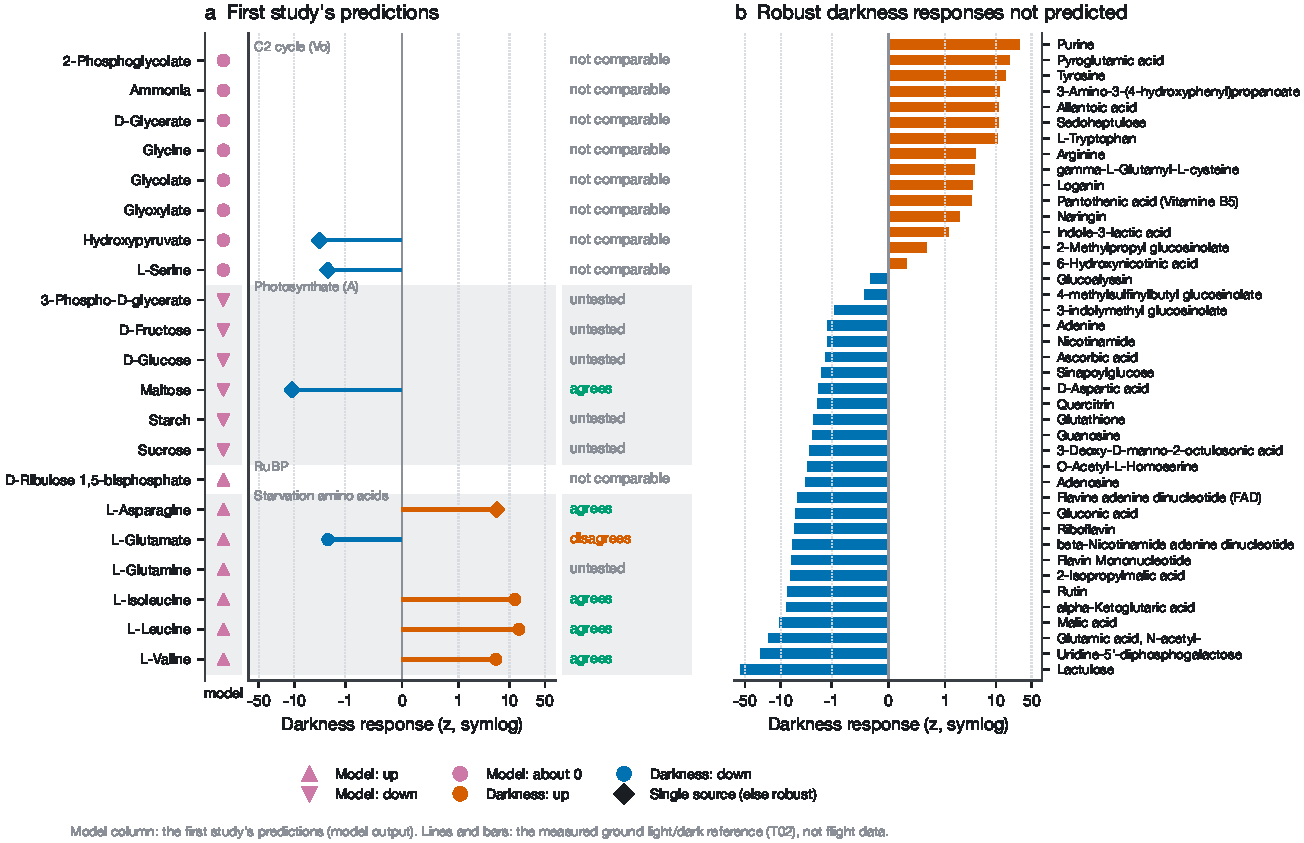
\includegraphics[width=\textwidth]{fig01_model_vs_reference.pdf}
\caption{\textbf{The first study's metabolite predictions set against measured darkness.}
\textbf{a}, The 21 predicted compounds, grouped by the model's driver. The model column gives the
predicted direction in OSD-522 (model output); lines give the measured light/dark response as a
standardised effect (T02; circles robust, diamonds single source). Verdicts follow the
pre-registered rule (Methods); C$_2$-cycle and RuBP predictions cannot be tested by darkness.
``Not measured'' and ``no direction'' are both untested: the first has no reference row, the second
was measured without a directional response. The glutamate call rests on the 32\,\textdegree C
source only (Supplementary Table~S2).
\textbf{b}, Robust darkness responses the model did not predict.}
\label{fig:model}
\end{figure}

\subsection{A measured metabolite layer leaves the pathway result unchanged}

We replaced the first study's metabolite layer in PaintOmics with the reference: all \nLayer{}
compounds, each valued at the model's own carbon-deficit magnitude (0.13\,log$_2$) in its measured
direction (0 for compounds without one), with the \nLayerRelevant{} robust compounds marked as
changed. PaintOmics takes a metabolite layer as two files, a table of compound name and value and a
list of ``relevant'' compounds; the relevant list is what its hub test uses. The gene and protein files
were byte-identical to the first study's job, and the database, organism and settings unchanged
(Methods). The layer is a ground reference, not a flight measurement: it says what carbon
starvation does to these compounds, which is what the model claims lit flight is.

The pathway result did not move (Fig.~\ref{fig:paint}a). The same \nPathA{} of \nPathTotal{}
pathways passed a Benjamini--Hochberg false discovery rate \citep{bh1995} of 0.05 in both jobs, led
in both by protein processing in the endoplasmic reticulum (combined $p \pErA$). The rank
correlation of all combined $p$-values was \rhoOneA{}. Glyoxylate and dicarboxylate metabolism,
where the C$_2$ cycle sits, moved from rank \rankGlyOne{} to \rankGlyA{}, still far from
significance.

The metabolite hubs changed only where the compound list changed (Fig.~\ref{fig:paint}b). Leucine,
valine, isoleucine and glutamate remained hubs, and malate, 2-oxoglutarate, glutathione,
ascorbate, glucobrassicin, $\gamma$-glutamylcysteine and 2-isopropylmalate joined them
(\nHubA{} hubs from \nHubTestedA{} compounds, against \nHubOne{} from \nHubTestedOne). The
pre-registered check held: for every compound and step the two jobs share, the raw hub $p$-value was
identical (\nSharedHubSteps{} compound-steps). PaintOmics returned a hub result for
\nRelevantTested{} of the \nLayerRelevant{} relevant compounds; the other \nRelevantNoHub, among them
glucosinolates, flavonoids, purine and sedoheptulose, got none (listed in Supplementary Table~S10).

Two post hoc control jobs test how far this goes (Supplementary Table~S10). Without any metabolite
layer (job E, K3ju047ZWB) the same \nPathE{} pathways passed (rank correlation \rhoAE). With each
compound valued at its own measured effect size, rescaled to the same median (job F, L46ds55AiY),
the pathway ranks did not change ($\rho = \rhoAF$), the same \nHubF{} hubs passed, and every raw hub
$p$-value was identical (\nSharedHubStepsF{} compound-steps). Across pathways the combined $p$
followed the gene $p$ ($\rho = \rhoCombGene$) more closely than the protein ($\rhoCombProt$) or
metabolite $p$ ($\rhoCombMet$; \nPathMetP{} pathways have one). Hub status, by contrast, needed both
gene-product layers: with genes alone (job G) or proteins alone (job H) and the same layer, none of
job A's \nHubA{} hubs remained. In this integration the gene-product layers decide the outcome, and
the metabolite layer contributes its list of relevant compounds, not their values.

\begin{figure}[t]
\centering
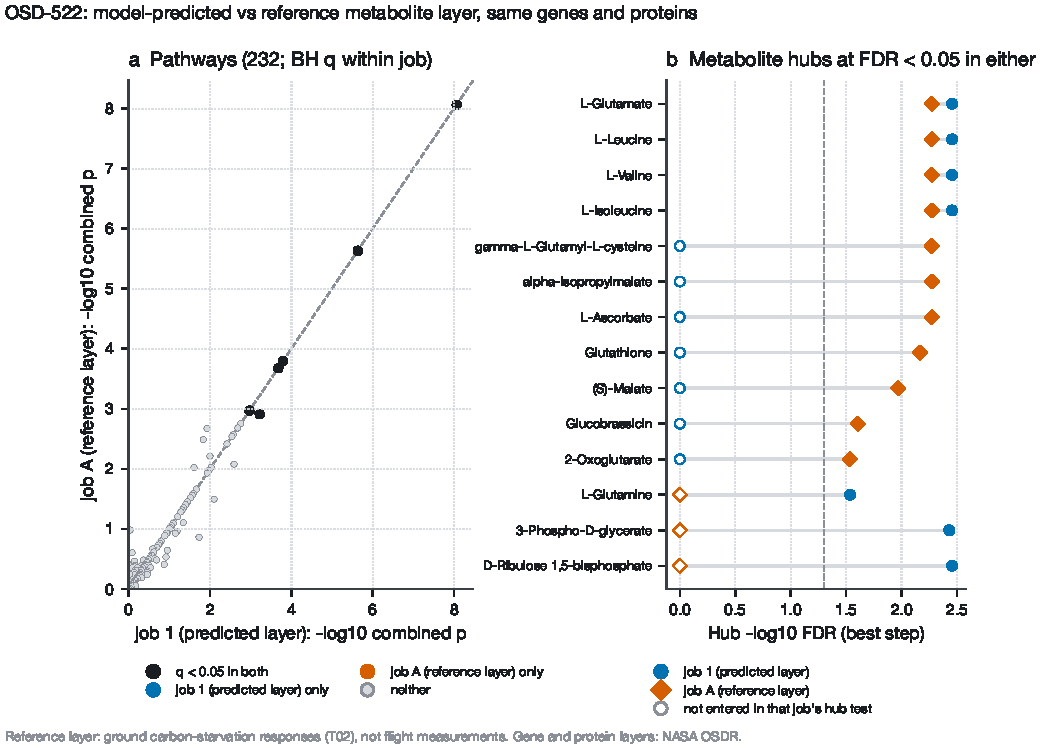
\includegraphics[width=\textwidth]{fig02_jobA_vs_job1.pdf}
\caption{\textbf{Replacing the predicted metabolite layer with the measured reference.} OSD-522
genes and proteins are identical in both jobs (first study oK2h66740Q, job A 6kBOS7AN5K). \textbf{a}, Combined Fisher $p$ for all
\nPathTotal{} pathways; colours mark BH $q<0.05$. \textbf{b}, Metabolite hubs at FDR $<0.05$ in
either job; open symbols mark compounds not entered in that job's hub test.}
\label{fig:paint}
\end{figure}

\subsection{Light and dark flight in the same hardware}

OSD-678 \citep{osd678} grew Col-0 seedlings in the same CARA plates on the same flight, either in
the ambient light of the station's cabin wall (4--6\,$\mu$mol\,m$^{-2}$\,s$^{-1}$) or wrapped in
black-out cloth from germination, which makes it the one place where light can be compared without changing hardware,
genotype or mission. We submitted both of its gene layers with the same reference metabolite layer
(Fig.~\ref{fig:lightdark}; jobs B, JfVZ1L37PY, and C, wgT3IPi7U2). The light contrast had more differentially expressed genes than the
dark one (\nDELight{} against \nDEDark{} at an adjusted $p<0.05$) and more significant pathways
(\nPathB{} against \nPathC{}); the two contrasts' pathway rankings were only moderately related
(rank correlation \rhoBC). Photosynthesis was the most significant pathway in the dark contrast
($p \pPhotoC$) and did not pass correction in the light one ($q \qPhotoB$). Valine, leucine and
isoleucine degradation was nominally significant in the dark ($p \pBcaaDegC$) and not in the light
($p \pBcaaDegB$).

In the light contrast \nHubB{} metabolite hubs reached FDR $<0.05$, against \nHubC{} in the dark. The
branched-chain amino acids, glutamate and 2-oxoglutarate were hubs only in the light, which is the
direction the model expects, but every light hub sat at the same adjusted value (\hubLightFDR) just
inside the threshold. That is the Benjamini--Hochberg step-up at work: it gives one adjusted value to
raw $p$-values from $\hubRawMinB$ to $\hubRawMaxB$ (Supplementary Table~S11). The five shared hubs
(malate, FAD, FMN, NAD$^+$ and 2-isopropylmalate) were stronger in the dark.

The light contrast also had \ratioDE{} times as many differentially expressed genes to place around
its hubs, so we cut its relevant genes at random to the dark contrast's number (post hoc, two draws,
jobs K1 Y0V56yFW12 and K2 7725j3CkOp). No hub survived in either draw, and \nPathKOne{} and
\nPathKTwo{} pathways passed, against \nHubC{} hubs and \nPathC{} pathways in the dark: the light
contrast's extra hubs come from its extra genes. To compare the flight effect between light regimes
without two separate thresholds, we fitted one model to the twelve Col-0 samples (edgeR TMM and
limma-voom \citep{robinson2010,law2014,ritchie2015}, flight $\times$ light; post hoc; Supplementary
Table~S9) and tested the interaction statistic with the rotation null. The model expects the
starvation sets to respond more to flight in light. They did not: the interaction was null for the
DIN set ($z = \zIntDin$) and for branched-chain catabolism ($z = \zIntBcaa$). It was large for the
photosystem and light-harvesting set ($z = \zIntPhoto$, $q \qIntPhoto$) and for the four KEGG
carbon pathways ($z$ from $\zIntFix$ to $\zIntSta$), because flight raised photosynthesis genes in
darkness ($z = \zLimmaPhotoDark$) and lowered them in light ($z = \zLimmaPhotoLight$).

\begin{figure}[t]
\centering
\includegraphics[width=\textwidth]{fig03_light_vs_dark.pdf}
\caption{\textbf{OSD-678 light and dark flight contrasts with the same reference layer.}
PaintOmics jobs B (JfVZ1L37PY, light) and C (wgT3IPi7U2, dark). \textbf{a}, Combined Fisher $p$ for
all pathways; the four most separated single-contrast pathways on each side are named.
\textbf{b}, Metabolite hubs at FDR $<0.05$ in either contrast; the light hubs share one
Benjamini--Hochberg value (raw $p$ in Supplementary Table~S11).}
\label{fig:lightdark}
\end{figure}

\subsection{Pre-registered light/dark gene-set tests}

Before any gene-set statistic was computed on a flight contrast, we committed six gene sets, the
predicted outcome for each in lit and dark flight contrasts, and every test setting
(prereg/PREDICTIONS.md; Table~\ref{tab:sets}). Two sets are signed: the first study's
carbon-starvation (DIN) set, re-tested here, and KEGG's valine, leucine and isoleucine degradation
pathway (\nSetBcaa{} genes), the catabolic route of the strongest darkness response. Four come from
the Wu GWAS: genes in loci found only under control, only under the darkness stress, under both,
and in the loci of metabolites with a directional darkness response. For OSD-522 the null was every
one of the 924 ways to relabel its twelve samples. The other five contrasts were tested on GeneLab's
published statistics, with too few replicates for a useful sample permutation (three per arm in
OSD-38 and OSD-678) or samples that could not be assigned to an arm from their names, so their null
was a genomic rotation that moves a set along the genome and keeps its size and clustering
(Methods).

Of the \nTests{} outcomes, \nMatch{} matched (Fig.~\ref{fig:sets}), but the matches are not where the
model needs them. In the lit contrasts none of the predicted signals passed correction:
\nLitMatch{} of \nLitTests{} lit outcomes matched, all of them comparator sets predicted to stay
flat. The DIN set leaned upward in all three lit contrasts (OSD-522 $p \pDinFiveTwoTwo$, OSD-678
light $p \pDinLight$, OSD-427 $p \pDinFourTwoSeven$; $q \ge \qDinFiveTwoTwo$ throughout), and so did
branched-chain catabolism in OSD-678 light ($p \pBcaaLight$, $q \qBcaaLight$). For OSD-522 the
first study had reported the DIN set at $p \pDinFirstStudy$ by Mann--Whitney, and the same test
here reproduces that value; under the sample permutation, which keeps the correlation between
genes, it weakens to $p \pDinFiveTwoTwo$.

The dark contrasts carried the strongest signals of all, where the model predicts none. The DIN
set fell in both BRIC-PDFU experiments (OSD-38 \citep{osd38}, $q \qDinThirtyEight$; OSD-321
\citep{osd321}, $q \qDinThreeTwoOne$) and rose in the leaves of dark-grown CARA seedlings (OSD-678 dark,
$q \qDinDark$). Branched-chain catabolism followed it, down in OSD-321 ($q \qBcaaThreeTwoOne$) and up
in OSD-678 dark ($q \qBcaaDark$). The natural-variation GWAS sets gave nothing light-specific: the
stress-only and darkness-metabolite loci were never enriched after correction, and the one
significant enrichment, of shared loci in OSD-678 light ($q \qSharedLight$), was in a comparator
set the model makes no claim about.

Post hoc diagnostics qualify these calls (Supplementary Tables~S5--S8, Figs~S2 and S3). The
rotation null is calibrated: on \nCalSets{} random gene sets and contiguous genomic blocks of 5 to
2{,}000 genes across the six contrasts it rejected a median \typeOneRotRandom{} of random sets and
\typeOneRotBlock{} of blocks at $\alpha = 0.05$ (range \typeOneRotMin--\typeOneRotMax), while a
naive random-gene null rejected up to \typeOneNaiveBlockMax{} of blocks, the inflation that gene
clustering causes. Sample permutation cannot confirm the 3-versus-3 contrasts: with 20 labellings
its smallest $p$ is 0.1, which the DIN set reached in OSD-38 ($p = \permDinThirtyEight$) but not in
OSD-678 dark ($p = \permDinDark$), where one of the three flight samples carries the rise
(Supplementary Table~S8). No single DIN gene drives the set: leaving out each in turn kept it
significant in OSD-38, OSD-321 and OSD-678 dark (largest $p = \looMaxThirtyEight$). Mixing pipelines
does not explain the dark results either: PyDESeq2 run on OSD-38's raw counts, as for OSD-522,
agreed with GeneLab's statistics (Spearman \pipeRhoStat{} over \pipeGenes{} genes), and the DIN fall
strengthened ($p \pDinThirtyEightDeseq$).

\begin{table}[t]
\caption{\textbf{Pre-registered gene sets and predictions.} Statistic: signed sets test the mean
gene statistic, unsigned sets the mean absolute statistic, each against the rest of the genome.
Lit contrasts: OSD-522, OSD-678 light, OSD-427. Dark: OSD-38, OSD-321, OSD-678 dark. Members are
in \texttt{prereg/gene\_sets.tsv}; all 36 results, with set statistic, $z$, $p$ and $q$, are in
Supplementary Table~S5.}
\label{tab:sets}
\begin{tabularx}{\textwidth}{@{}lrXlll@{}}
\toprule
Set & Genes & Definition & Statistic & Lit & Dark\\
\midrule
DIN (first study) & \nSetDin & KEGG gene descriptions matching DIN$n$, the first study's rule & signed & up & none\\
BCAA degradation & \nSetBcaa & KEGG ath00280 & signed & up & none\\
Wu stress-only & \nSetWuStress & Genes of GWAS regions found only under 32\,\textdegree C darkness & unsigned & enriched & none\\
Wu darkness metabolites & \nSetWuDarkMet & Loci of metabolites with a directional darkness response & unsigned & enriched & none\\
Wu control-only & \nSetWuControl & Genes of GWAS regions found only under control & unsigned & none & none\\
Wu shared & \nSetWuShared & Genes of GWAS regions found under both & unsigned & none & none\\
\botrule
\end{tabularx}
\end{table}

\begin{figure}[t]
\centering
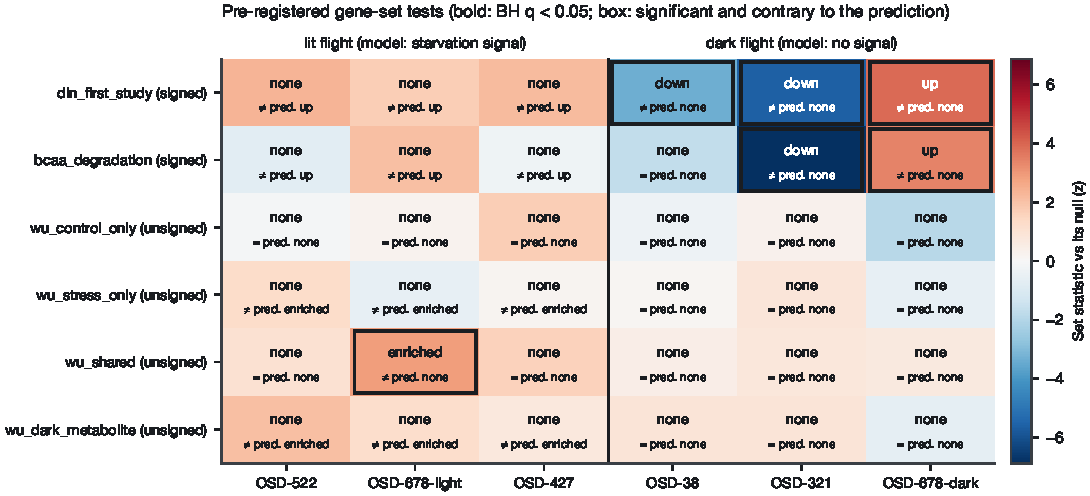
\includegraphics[width=\textwidth]{fig04_geneset_tests.pdf}
\caption{\textbf{Pre-registered light/dark gene-set tests.} Colour: the set statistic against its
null as a $z$-score (OSD-522, sample permutation; others, genomic rotation). Each cell gives the
observed outcome (bold where BH $q<0.05$ over the \nTests{} tests) and whether it equals ($=$) or
contradicts ($\neq$) the prediction; boxes mark significant contradictions.}
\label{fig:sets}
\end{figure}

\subsection{What a targeted GC-MS panel would need}

To ask whether the predicted metabolite shifts could be measured on archived flight material, we
estimated per-compound replicate variance from Col-0 wild-type control groups in MetaboLights GC-MS
studies \citep{yurekten2024}: \nPanelGroups{} groups in \nPanelStudies{} studies
\citep{sanchez2008,abraham2016,fabregas2018,zhang2022}, \nPanel{} compounds from the model's
predictions and the reference (Fig.~\ref{fig:power}). The median within-group standard deviation of
log$_2$ intensity ran from \sdMin{} (sucrose) to \sdMax{} (isoleucine).

With six plants per arm, OSD-522's RNA-seq design, the smallest change detectable at 80\,\% power
was \detectMin{} log$_2$ (\detectMinFold-fold), for sucrose. The model's predicted 0.13\,log$_2$
shift would need \nQThousandMin{} to \nQThousandMax{} plants per arm, and its \qSixtyLogTwo\,log$_2$
shift at OSD-522's own growth light at least \nQSixtyMin{}. A two-fold change, the scale of the
measured darkness responses, would need at most \nTwoFoldMax{}. A panel tests many compounds at once; with Bonferroni correction over the \nPanel{} compounds the smallest detectable change at
six per arm rose to \detectMinBonf{} log$_2$ (\detectMinFoldBonf-fold), 0.13\,log$_2$ would need
\nQThousandBonfMin{} to \nQThousandBonfMax{} plants per arm, and a two-fold change at most
\nTwoFoldBonfMax{} (Fig.~\ref{fig:power}, open symbols). The variance sources are listed in
Supplementary Table~S14. One of them, MTBLS363, is the deposit of a CAM study in
\textit{Agave} \citep{abraham2016} that also profiled an untreated \textit{Arabidopsis} Col-0
day--night series; only that \textit{Arabidopsis} assay (\nMtblsThreeSixThreeGroups{} timepoints,
\nMtblsThreeSixThree{} rosettes) was used.

\begin{figure}[t]
\centering
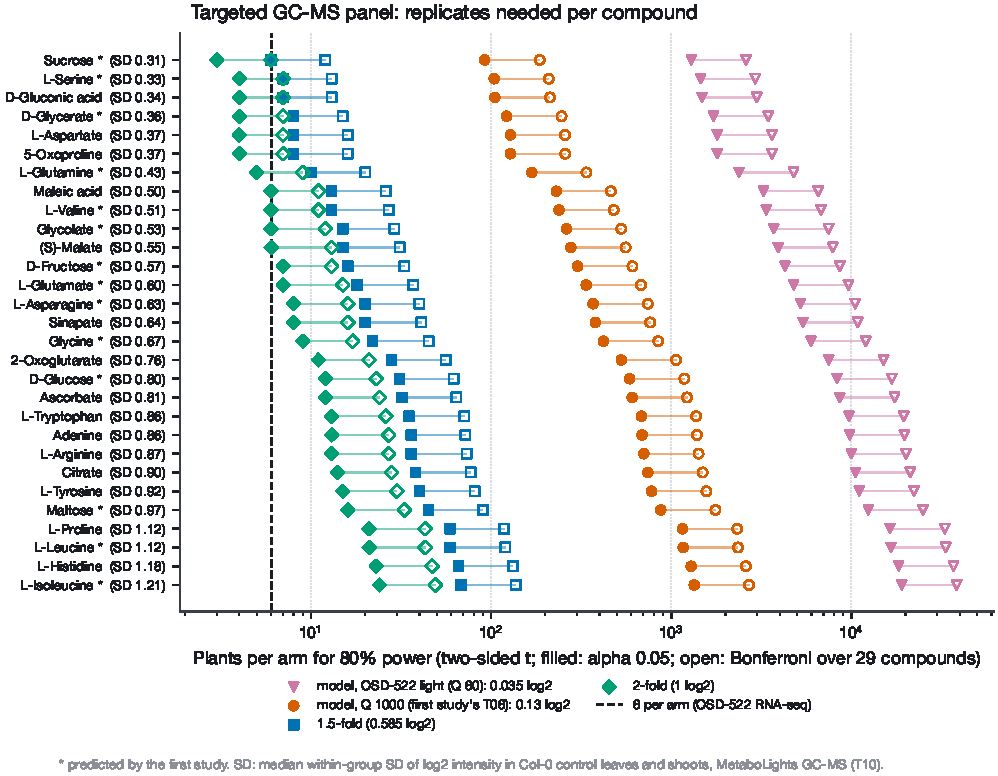
\includegraphics[width=0.92\textwidth]{fig05_gcms_power.pdf}
\caption{\textbf{Plants per arm for a targeted GC-MS panel.} Two-sided two-sample $t$-test, 80\,\%
power; filled symbols $\alpha=0.05$ unadjusted, open symbols Bonferroni over the \nPanel{}
compounds. Effects: the model's OSD-522 shift (\qSixtyLogTwo\,log$_2$) and its 0.13\,log$_2$, 1.5-fold
(0.585\,log$_2$) and two-fold. Variance from Col-0 control groups in MetaboLights GC-MS studies
(Supplementary Table~S14). Asterisks mark compounds the first study predicted.}
\label{fig:power}
\end{figure}

\subsection{A dark sealed BRIC with a proteome}

OSD-38 (BRIC-20) grew Col-0 seedlings for about three days in darkness on 0.5x MS with 1\,\%
sucrose, in sealed BRIC-PDFU canisters on the station and on the ground, and measured their
transcriptome and the iTRAQ proteomes of a membrane and a soluble fraction \citep{osd38,kruse2020}.
The same study holds a GeneLab ground comparator: on the ground, 22 plates were sealed in PDFUs
inside BRIC canisters at Kennedy Space Center and 22 were wrapped in foil in opaque, air-tight plastic
containers at Ohio University; both sets were held cold for 4 days, grown for 76\,h in darkness and
fixed in RNAlater, and GeneLab's contrast compares three samples of each \citep{osd38,basu2017}.
The two arms differ in hardware, site and handling, so we read it as a comparator, not as an isolated
hardware effect. We added both under a second pre-registration, committed before any
OSD-38 protein or hardware statistic was computed (\texttt{prereg/osd38/}). It covers nine gene
sets in four layers; the first study's model predicts no signal for any of them in dark flight.

OSDR's processed protein tables are truncated. Both the CSV and the spreadsheet copies stop at
\nOsdRows{} data rows, the old spreadsheet row limit, and OSDR lists one version of each, from 2017
(Supplementary Table~S12). The membrane table holds two acquisitions in sequence; the first
(\nMemGroups{} protein groups, numbered up to \nMemGroupMax) ends before the cut and was used whole,
giving \nProtMem{} quantified proteins. The soluble table stops inside its 438th protein group, so
only groups 1--\nSolGroups{} could be used, as a secondary layer; they hold \nSolLoci{} loci,
because \nSolTwoGroups{} loci occur in two groups, and no locus was lost to the filters. Quantified by the paper's rules, the membrane layer
gave \nPaperRule{} proteins at the paper's threshold, against the 103 the paper reports
\citep{kruse2020}.

In OSD-38, transcripts and proteins of carbon metabolism moved in opposite directions
(Fig.~\ref{fig:osd38}). All four KEGG carbon pathways rose in the transcriptome (glyoxylate and
dicarboxylate, carbon fixation, starch and sucrose, glycolysis; $q \le \qRnaCarbonMax$), as did the
photosystem and light-harvesting set ($z = \zRnaPhoto$), while the DIN set fell ($z = \zRnaDin$);
these transcript rows re-test what the first study reported. In the membrane proteome the same four
pathways fell in the membrane fraction ($z$ from $\zMemSta$ to $\zMemGlyc$, $q$ from $\qMemCarbonMin$
to $\qMemCarbonMax$). This held against random protein sets matched for abundance (PSM count; $p$
from $\pRobMin$ to $\pRobMax$), the protein statistic was unrelated to abundance
($\rho = \rhoPsm$), and a moderated (limma) $t$ gave the same verdicts ($q$ from $\qLimmaCarbonMin$
to $\qLimmaCarbonMax$; post hoc, Supplementary Table~S12). Whether this reflects how much of each
enzyme the seedlings made, or how it partitioned into the 100{,}000\,$g$ membrane pellet, these
tables cannot say: for the \nPartition{} proteins quantified in both fractions, membrane and soluble
fold changes were unrelated ($\rho = \rhoPartition$), and carbon-pathway members in the soluble
subset were not lower in flight (mean log$_2$ fold change \solCarbonFcMin{} to \solCarbonFcMax). The
protein result therefore applies to the membrane fraction.
Branched-chain amino acid degradation, the catabolic route of the strongest darkness response, did
not move in either layer ($z = \zRnaBcaa$ for transcripts and $\zMemBcaa$ for \nMemBcaa{} membrane
proteins). The DIN, fermentation, hypoxia and photosystem sets had too few measured proteins to
test. Across all proteins, protein and transcript changes were only weakly correlated
($\rho = \rhoMem$ for the membrane fraction, $\rhoSol$ for the soluble subset; $\rhoFiveTwoTwoProt$
over \nFiveTwoTwoProt{} proteins in OSD-522). The truncated soluble subset showed no significant
set.

In the ground comparator, the pre-registered hypoxia and fermentation sets did not rise in the
BRIC-PDFU against the air-tight container ($z = \zHwHyp$ and $\zHwFer$), the outcome derived from
the first study's enclosure mass balance. Carbon fixation and glyoxylate and dicarboxylate
metabolism rose in the BRIC ($q \qHwFix$ and $\qHwGly$) and starch and sucrose fell ($q \qHwSta$).
Of the \nOsdTests{} testable primary OSD-38 outcomes, \nOsdMatch{} matched the predictions.

A positive control shows that this null is partly uninformative (post hoc; Supplementary
Table~S13). In three independent hypoxia datasets, Ws roots at low oxygen under hypobaria
\citep{osd136,zhou2017} and Col-0 shoots and roots after 2\,h of hypoxia
\citep{mustroph2009,gse14502}, the fermentation set rose strongly ($z = \zFerOsdOneThreeSix$,
$\zFerShoot$ and $\zFerRoot$), but the hypoxia-responsive set, defined by gene annotation and with
\nHypMeasured{} of its \nHypSet{} genes on the array, did not respond to hypoxia at all, so its null
in the comparator says nothing. The fermentation set's null, in turn, hides its strongest member:
pyruvate decarboxylase PDC1 rose \foldPdcHw-fold in the BRIC ($q \padjPdcHw$) while the set's other
genes did not, and alcohol dehydrogenase ADH1, which is not in the set, rose \foldAdhHw-fold. We
therefore added, after seeing these results, a signature from independent data (an addendum to the
revision plan, committed before it ran): the \nHypUp{} genes up more than two-fold in both
GSE14502 tissues. It rose in OSD-136 ($z = \zHypUpOsdOneThreeSix$) and rose strongly in the
BRIC-PDFU against the container ($z = \zHypUpHw$, $q \qHypUpHw$), while the matching down signature
fell ($z = \zHypDownHw$). On the ground, seedlings in the sealed BRIC-PDFU carry the transcript
signature of low oxygen relative to the air-tight container. In flight against ground, both in
BRIC-PDFU, the signature was slightly lower in flight ($z = \zHypUpFlight$, $q \qHypUpFlight$).
Across all genes, the flight effect was weakly anti-correlated with the comparator effect
($\rho = \rhoFlightHw$; exploratory).

Submitted to PaintOmics with the same reference layer (job D), OSD-38's genes and membrane
proteins gave \nPathD{} pathways at FDR $<0.05$, against \nPathA{} for OSD-522's lit canister
(job A). Only \nPathAD{} pathway was shared, and the rank correlation was $\rhoAD$
(Fig.~\ref{fig:bric}). Of the metabolite hubs, \nHubAD{} were shared by the lit and the dark
canister: leucine, isoleucine, glutamate, malate, 2-oxoglutarate and 2-isopropylmalate. The first
study read these hubs as signs of lit-canister starvation; they appear in the dark too. The overlap
is no larger than chance, however (post hoc; Supplementary Table~S11). Two hub sets of these sizes
drawn from the same \nHubCand{} tested compounds share \hubOverlapExp{} on average
(hypergeometric $P(\ge\nHubAD) = \hubOverlapP$), or \hubOverlapExpPerm{} with hub labels shuffled
within tertiles of KEGG reaction count ($P = \hubOverlapPPerm$), and hubs did not have more KEGG
reactions than other tested compounds in any job (Mann--Whitney $p \ge \mwDegreePMin$). Job D's
hubs largely survived with genes alone (\nHubI{} of \nHubD, job I) and vanished with membrane
proteins alone (job J). Hub calls therefore do not separate the lit from the dark canister.

\begin{figure}[t]
\centering
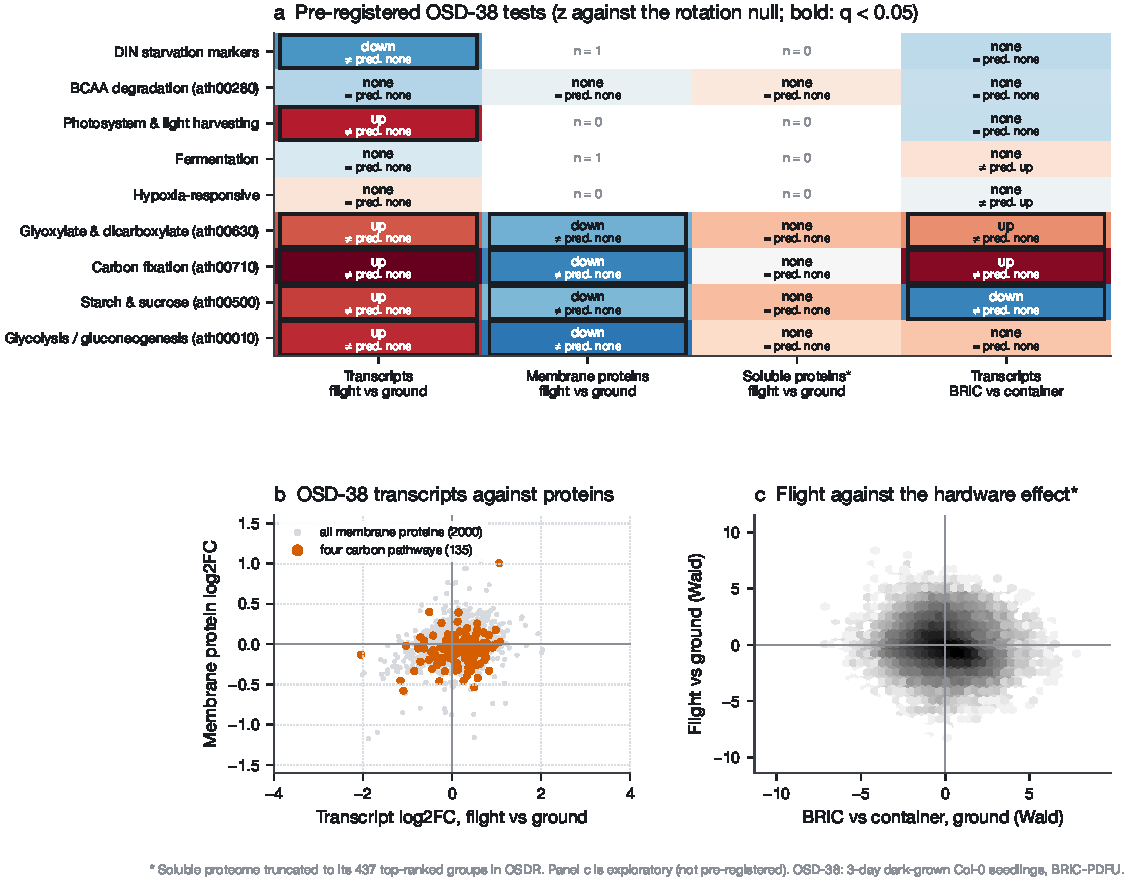
\includegraphics[width=\textwidth]{fig06_osd38.pdf}
\caption{\textbf{OSD-38: a dark sealed BRIC with a proteome.} \textbf{a}, Pre-registered gene-set
tests in four layers ($z$ against the rotation null; bold where BH $q<0.05$; boxes mark significant
contradictions of the prediction; $n$ = measured members where fewer than three). The soluble
proteome is the 437 top-ranked groups left in OSDR's truncated table. \textbf{b}, Transcript
against membrane-protein log$_2$ fold change, flight vs ground; red, members of the four KEGG
carbon pathways. \textbf{c}, Exploratory: the flight effect against the GeneLab ground comparator (BRIC-PDFU vs
air-tight container), all genes.}
\label{fig:osd38}
\end{figure}

\begin{figure}[t]
\centering
\includegraphics[width=\textwidth]{fig07_bric_lit_vs_dark.pdf}
\caption{\textbf{Sealed BRIC, lit (OSD-522, job A 6kBOS7AN5K) against dark (OSD-38, job D
Es6j23q40o).} Both jobs carry genes, proteins and the same ground reference metabolite layer. The
\nHubAD{} shared hubs are no more than two hub sets of these sizes share by chance (Supplementary
Table~S11). \textbf{a}, Combined Fisher $p$ for
all pathways. \textbf{b}, Metabolite hubs at FDR $<0.05$ in either job.}
\label{fig:bric}
\end{figure}

\section{Discussion}\label{sec:discussion}

\subsection{Compared with the first study}

Table~\ref{tab:compare} sets the two studies side by side. The measured data support the model's
metabolic picture in outline: under extended darkness the branched-chain amino acids and asparagine
rise and maltose falls, as it predicted, at every threshold we tried. They correct it in detail.
Glutamine does not move, the starvation amino acids differ several-fold in how strongly they
respond, and the TCA-cycle acids the model declined to predict fall consistently. Glutamate falls
only in the 32\,\textdegree C source, so whether it contradicts the model is open. None of this
tests the gas-transport mechanism itself: darkness cannot score the C$_2$-cycle and RuBP
predictions that carry it.

The light/dark prediction fares worse. The model's mechanism runs through photosynthesis, so its
signature should appear in light and vanish in the dark. With nulls that respect gene correlation
and predictions fixed in advance, no lit contrast produced a significant starvation signal, while
three dark contrasts produced the strongest ones in the dataset, and a single model of OSD-678
showed no larger starvation response to flight in light than in darkness. The first study reported that its
starvation-over-photosynthesis contrast separated lit from dark experiments; a single-set test shows
why that ordering is not a light effect. The starvation genes themselves move most in darkness, in
opposite directions in BRIC-PDFU seedlings and in CARA leaves.

\begin{table}[t]
\caption{\textbf{The first study and this one, claim by claim.}}
\label{tab:compare}
\begin{tabularx}{\textwidth}{@{}XXX@{}}
\toprule
Claim & First study \citep{firststudy} & This study\\
\midrule
Starvation amino acids rise together & Predicted together, one shared gain of 1, unfitted & Leu, Ile, Val, Asn rise; Glu falls in the 32\,\textdegree C source only; Gln has no direction; Leu responds \ratioLeuAsn--\ratioLeuVal{} times as strongly as Val or Asn\\
TCA-cycle acids & Not predicted (direction uncertain) & Malate and 2-oxoglutarate fall robustly, each in two sources\\
Metabolite layer in PaintOmics & \nModelCompounds{} predicted compounds & \nLayer{} measured compounds, no layer or rescaled values: pathways unchanged; hubs need genes and proteins together\\
Lit flight shows a starvation signal & DIN up in OSD-522 ($p \pDinFirstStudy$, Mann--Whitney) & Leans up in all three lit contrasts; none significant after correction under gene-correlation-aware nulls\\
Dark flight shows none & Predicted none; dark inversions unexplained & Strongest signals are in dark-grown seedlings (gene-level null; too few plants for sample permutation); sign differs between BRIC canisters and CARA plates\\
Metabolite shifts are measurable & Proposed a 20--30 compound panel on archived material & Needs \nQThousandMin--\nQThousandMax{} plants per arm for 0.13\,log$_2$\\
Transcripts stand in for metabolism & Read pathways and hubs from transcripts & In dark BRIC flight (OSD-38) carbon-pathway transcripts rise while the same enzymes fall in the membrane fraction\\
Starvation hubs mark the lit canister & Seven hubs at FDR $<0.05$, all starvation or supply nodes & Six of them are hubs in the dark BRIC too, an overlap no larger than chance; hub calls follow gene counts\\
Enclosure atmosphere matters & Mass balance: a dark BRIC loses O$_2$ over days & Ground comparator: pre-registered sets null, but an independent low-oxygen signature rises strongly in the BRIC-PDFU (post hoc)\\
\botrule
\end{tabularx}
\end{table}

\subsection{What a proteome adds}

Both the first study's starvation reading and every PaintOmics integration here read metabolism
from gene products, mostly transcripts. OSD-38 is the one dark sealed-BRIC flight with a proteome, and there the carbon
pathways' transcripts rose while their proteins fell in the membrane fraction; the soluble subset did
not follow, so the result may reflect how these enzymes partition between fractions as much as how
much of them was made. Kruse et al.\ saw the same decoupling
gene by gene: nearly 30\,\% of the 17 genes that changed at both levels moved in opposite
directions, and they pointed to post-transcriptional regulation \citep{kruse2020}. At the pathway
level it means a transcript signature is not a reliable proxy for the enzyme complement, and still
less for metabolite pools. The hub result points the same way. The branched-chain amino acid and
glutamate hubs that the first study attributed to a lit-canister carbon deficit appear in a dark
canister with no assimilation to lose, at an overlap no larger than chance, and in OSD-678 the light
contrast's hubs disappeared when its gene list was cut to the dark contrast's length. Hub status
reflects how many genes change around a compound in the network, not why they change.

\subsection{Why the dark contrasts carry the signal}

We cannot say from these data, and offer possibilities to test rather than conclusions. In all
three dark contrasts both arms are seedlings grown in darkness from germination
\citep{osd38,osd321,osd678}, so the flight-versus-ground contrast compares two starved states, and
a difference in the starvation programme means the flight seedlings were starved more, less or
differently than their ground controls. The direction is not consistent: the programme is lower in
flight in the two BRIC-PDFU canister experiments and higher in the CARA plates, which differ in
hardware (a sealed canister against a plate on the cabin wall) and in what was sequenced (whole
seedlings against dissected leaves). Either way, a carbon-starvation programme responds to
spaceflight conditions that the boundary-layer mechanism cannot reach, because in the dark there
is no assimilation for it to reduce. OSD-38's seedlings also grew on 1\,\% sucrose (OSDR protocol),
which makes classical carbon starvation unlikely in either of its arms and leaves the cause of its
DIN fall open. One candidate is oxygen. On the ground, seedlings in the sealed BRIC-PDFU carried a
low-oxygen transcript signature relative to an air-tight container, and in flight that signature
was slightly weaker than in the ground BRIC. The DIN set itself rose under hypoxia in the
GSE14502 roots ($z = \zDinRoot$), so the dark contrasts may compare two oxygen states as well as two
carbon states. These signals also rest
on gene-level nulls: with three plants per arm, sample permutation cannot confirm them, and in the
OSD-678 dark contrast one flight sample carries the DIN rise.

\subsection{Limitations}

The reference is ground darkness, a far larger perturbation than a 9\,\% assimilation deficit and
one that also starts senescence and nitrogen remobilisation, so it fixes directions rather than
flight magnitudes, and its use as a stand-in for flight rests on the first study's hypothesis. The
sources differ in age, tissue, photoperiod, sampling time and platform (Table~\ref{tab:sources}),
Zhu's papers do not state the temperature in darkness, and Wu's time-course columns are labelled 20
and 30 where its text gives 21 and 32\,\textdegree C. The Caldana plants are Col-0 according to the
authors' deposit \citep{emtab375} and Wu et al.\ \citep{wu2018}; we could not read the Caldana paper
itself. The reference covers secondary metabolism poorly, because specialised metabolites map to
KEGG poorly. Gene-set tests on GWAS regions include many genes that do not cause the association,
which dilutes any signal. The five contrasts other than OSD-522 were tested with a rotation null;
it is calibrated on random sets and genomic blocks, but it treats genes, not plants, as the unit,
and OSD-38 and OSD-678 have three replicates per arm, too few for a sample permutation to reach
significance. OSD-678's light arm was
the cabin's ambient light of 4--6\,$\mu$mol\,m$^{-2}$\,s$^{-1}$ \citep{osd678}, well below OSD-522's
60, where the model's deficit is smaller still, so its light/dark comparison is a weak test of the
model's light dependence. PaintOmics hub counts rise with the number of
differentially expressed genes, which differs \ratioDE-fold between the two OSD-678 contrasts; at
equal numbers the light contrast had no hubs.
The GC-MS variance pools leaf and shoot studies from different laboratories and timepoints.
OSDR's OSD-38 protein tables are truncated, so the soluble layer is a top-ranked subset and the
membrane layer one of two acquisitions; re-searching the raw iTRAQ files, which OSDR holds, would
recover the rest and is left for future work. iTRAQ compresses ratios, which shrinks protein fold
changes but should not reverse them. The membrane fraction is a 100{,}000\,$g$ pellet rather than
total protein, and the two fractions disagree, so the protein result is a statement about that
fraction. The GeneLab ground comparator differs in site (Kennedy Space Center against Ohio
University) and in handling as well as in enclosure, and the container's gas volume is not
reported \citep{osd38,basu2017}; its hypoxia signature locates the difference in oxygen but not its
cause. The pre-registration was written by the same analyst on the same day as the tests, after
the reference had been built; its value lies in the commit order, which shows that no prediction or
setting was changed after a flight result was seen. The revision analyses are post hoc: their plan
was committed before they ran, but after the pre-registered results were known, and the hypoxia
signature was added after the positive control had been seen.

\section{Methods}\label{sec:methods}

\textbf{Inputs and provenance.} Every input is vendored with its source and SHA-256 in
\texttt{data/*/PROVENANCE.md}. Derived natural-variation tables (Zhu per-accession darkness
responses, Wu leaf metabolomes with one ion mode per metabolite, Wu GWAS loci and condition
regions) and the OSD-522 raw counts are read from the Arabidopsis Atlas at commit 69b21c6
\citep{atlas}. The first study's PaintOmics upload, job record, predictions and study registry are
read from its repository at commit 515226d \citep{firststudy}. Per-contrast GeneLab
differential-expression statistics for OSD-38, OSD-321, OSD-678 light and dark and OSD-427
\citep{osd38,osd321,osd678,osd427} keep only the matched flight-versus-ground columns named in that
registry. The Wu supplementary tables 7 and 8 are fetched to a git-ignored cache and only derived
values are committed. Files added for the revision (OSDR OSD-38, OSD-136 and OSD-678 counts and
tables; GEO GSE14502 and GPL198) are fetched the same way, with their SHA-256 recorded in
\texttt{data/reference/revision1\_sources.tsv}.

\textbf{Light/dark reference.} Zhu: per-accession 6\,d minus 0\,d of the published BLUPs, which
have no missing or zero values, so every accession with both timepoints contributes (\nZhuAcc).
Wu: stress minus control per accession, one ion mode per metabolite (a mode measured in both
conditions where one exists); metabolites with no mode shared by the two conditions, or listed on
two rows of Wu's identification table, are excluded, and accessions missing either value are
dropped (median \wuMissMedian\,\% of the \nWuPossible{} accessions, at most \wuMissMax\,\%;
\wuNMin--\nWuAcc{} accessions per compound). Caldana (Wu supplementary table 7, whose column labels
20-D and 20-L we read as the 21\,\textdegree C dark and light conditions of the text): mean dark
minus light over the timepoints at or after 360\,min, three replicates each, values missing in an
arm dropped and at least three per arm required (\nCaldanaMin--\nCaldanaMax{} values per compound),
Welch $t$-test, peaks restricted to those Wu named with a KEGG identifier and, where several peaks
share one, the most intense kept. The script stops if any source has two rows for one KEGG compound.
Per-compound $n$ and missingness are in Supplementary Table~S2. A Zhu or Wu
response qualified when its median was non-zero, at least 75\,\% of at least 20 accessions moved in
its direction; a Caldana response qualified at $p<0.05$. Consensus: conflicting if qualifying
sources disagreed, robust if at least two agreed or one had at least 90\,\% of accessions, single
otherwise. The reference value is the mean standardised effect of the qualifying sources (response
divided by the source's SD across accessions or light replicates). Compound names were matched to
KEGG by the REST API, a name counting only when it equals a KEGG synonym after case, punctuation
and an L-/D- prefix are ignored; every candidate is recorded and every correction is listed with
the KEGG name that confirms it (\texttt{data/reference/kegg\_overrides.tsv}). Amino acids take
their L-forms, since LC-MS does not resolve enantiomers. The same overrides correct
\nOverCaldanaFix{} and exclude \nOverCaldanaExcl{} of the KEGG identifiers Wu gave the Caldana peaks.

\textbf{Compound rule.} Quoted from \texttt{prereg/settings.json} (\texttt{compound\_rule}, commit
858ca21): ``a T06 prediction whose driver is net assimilation (A) or carbon starvation is compared
with the T02 consensus direction: agrees if the signs match, disagrees if they differ, untested if
T02 has no directional status for that KEGG ID''; and ``Vo- and RuBP-driven predictions: darkness
stops oxygenation and carboxylation together, so a darkness reference cannot test them'' (not
comparable). A directional status is robust or single. T03 adds \texttt{verdict\_detail}, which
splits untested into not measured (no T02 row) and no direction (status none or conflicting)
without changing the verdict.

\textbf{Pre-registration.} \texttt{scripts/11\_prereg.py} wrote the gene sets, genome order,
settings and predictions to \texttt{prereg/}, committed alone (commit 858ca21) before any test script
existed; the test script reads those files and will not run without them. The DIN set was flagged as
a re-test, since the first study had already reported it in all six contrasts. Wu GWAS sets: Wu's
supplementary table 5 lists, for each locus with a SNP at $p<10^{-8}$ (LOD above 8), the genes
assigned to it; we take those gene lists as given (Wu do not state the window they used). The
\nWuLoci{} condition-by-mode loci were merged across conditions and ion modes into \nWuRegions{}
regions wherever their base-pair spans overlapped, a region's genes are the union of its loci's
genes, and a region is control-only, stress-only or shared by the conditions in which its loci were
found. KEGG gene lists and pathway memberships were retrieved on 30 October 2026 and frozen in
\texttt{prereg/gene\_sets.tsv}.

\textbf{Gene-set tests.} OSD-522 Wald statistics were recomputed from raw counts with PyDESeq2
\citep{pydeseq2,love2014}, six flight against six ground shoots, genes with a total count of at
least 10; the log$_2$ fold changes match the first study's upload to within $10^{-6}$. Its
permutation null used a Welch $t$ on log$_2$(median-of-ratios normalised count + 1) under all 924
labellings, the observed labelling included. The rotation null shifted each set's positions in the
KEGG genome order by 10{,}000 random offsets (seed 20261030). Two-sided $p$-values for signed sets,
upper-tail for unsigned; BH correction over the 36 primary tests. Before testing, the script plants
a shift into 60 genes and leaves 60 control genes untouched, and stops unless both nulls find the
first and not the second.

\textbf{PaintOmics.} Jobs were submitted to paintomics.org with organism \texttt{ath}, KEGG and
MapMan, and AI interpretation off, by the multipart request the web form makes; the matching step
was run in a browser, and the full job records were recovered and vendored. On each compound card,
matches were reduced to the intended KEGG identifier (PaintOmics also selected CMP-KDO,
neoglucobrassicin, sugar anomers and a non-KEGG NADP$^+$ identifier); one residual, (S)-allantoin on
a compound of value 0, is recorded. Uploads: a gene or protein table (identifier, log$_2$ fold
change) with a relevant list (adjusted $p<0.05$ for genes); for metabolites, a table of KEGG name and
value and a relevant list of the robust compounds. Hub results are each compound's best (lowest)
adjusted $p$ over PaintOmics' steps. Job identifiers: first study oK2h66740Q; A 6kBOS7AN5K; B
JfVZ1L37PY; C wgT3IPi7U2; D Es6j23q40o; revision controls E K3ju047ZWB, F L46ds55AiY, G
Y72ky4006o, H N2XgxyWlJn, I sD7V1nZ4t4, J C3kVBAm3N5, K1 Y0V56yFW12, K2 7725j3CkOp.

\textbf{OSD-38.} The processed iTRAQ tables (soluble and membrane, OSDR) were fetched with their
SHA-256 recorded. Membrane: rows of the first block only (groups 1--2{,}948); soluble: groups
1--437. Peptide-spectrum matches with score above 20 and all six reporter intensities positive were
kept, and loci with at least two distinct peptides, as in the paper \citep{kruse2020}. Each
channel was centred on its median, each match on its own mean, and a protein's channel value was
the median over its matches. Flight minus ground gives the log$_2$ fold change, tested with a
two-sided Student's $t$ (three against three). The pre-registration addendum
(\texttt{scripts/21\_prereg\_osd38.py}) fixed this method, the nine sets (DIN, BCAA degradation,
the first study's photosystem, fermentation and hypoxia rules, and KEGG ath00630, ath00710,
ath00500 and ath00010), the minimum of three measured members, the rotation null over measured
features and the predictions before any OSD-38 protein or hardware statistic existed. BH
correction ran over the testable primary rows (flight transcripts, membrane proteins, hardware
transcripts). The hardware contrast is GeneLab's ground BRIC-PDFU against closed-container plates,
both fixed in RNAlater. A planted-signal check on the membrane proteins precedes the tests.
Abundance robustness, not pre-registered, compares each membrane set with 5{,}000 random sets
matched on PSM-count decile. PaintOmics job D carried the OSD-38 genes (relevant at adjusted
$p<0.05$), membrane proteins (relevant at $p\le0.05$ and $|\log_2\mathrm{FC}|>0.2$, the paper's
rule) and the reference layer.

\textbf{Power.} Col-0 control groups: the 0\,mM salt group of MTBLS22, 41 and 42; Col-0
well-watered shoots of MTBLS2289 per timepoint; the wild-type group of MTBLS4066; the Col-0 time
course of MTBLS363 per timepoint. MTBLS8105 was excluded because its values carry commas whose
decimal convention cannot be determined, and the single-leaf series MTBLS7, 11, 12 and 13 because
leaf position is not recorded. Compounds were matched by KEGG's ChEBI conversion or by KEGG
synonym. Per compound, the median over groups of the within-group SD of log$_2$ intensity (zeros
missing, at least three values) set the required $n$ per arm for a two-sided two-sample $t$-test by
the noncentral $t$ distribution, at $\alpha = 0.05$ and with Bonferroni correction over the
\nPanel-compound panel. The Golm salt-series values are percentages of each compound's maximum in the
study, a per-compound rescaling that leaves log$_2$ SDs unchanged.

\textbf{Revision analyses (post hoc).} Written in \texttt{prereg/revision1/} (commit 90ff4b8, with an
addendum for the hypoxia signature in 8d6a9ae) before they ran, after the pre-registered results
were known; they add tables and do not change T02, T08, T12 or the T03 verdicts, which the scripts
check. Reference strata and sensitivity (\texttt{scripts/23}): the consensus rule within all three
sources, darkness only (Zhu, Caldana) and dark+heat (Wu), and over accession agreement of 60, 70, 75,
80 and 90\,\% crossed with Caldana windows from 60, 180 and 360\,min. Gene-set diagnostics
(\texttt{scripts/25}): 200 random gene sets and 200 contiguous genomic blocks at each of five sizes
per contrast, each tested against 999 rotation offsets and a naive random-gene null (seed
20261102); exact permutation over the 20 labellings of the 3-versus-3 contrasts, Welch $t$ on
log$_2$(GeneLab normalised count + 1); PyDESeq2 on OSD-38's raw RSEM counts with OSD-522's settings;
DIN gene by gene and with each gene left out. OSD-678 interaction (\texttt{scripts/24}): GLDS-612
rRNA-removed RSEM counts of the twelve Col-0 samples, genes with a total count of at least 10, edgeR
TMM \citep{robinson2010} and limma-voom \citep{law2014,ritchie2015} on the four flight-by-light
groups, the interaction contrast tested with the rotation null and BH over eleven sets. Hypoxia
positive control (\texttt{scripts/26}): GeneLab's OSD-136 limma $t$ for 50\,kPa without against
with oxygen restored to 21\,kPa \citep{osd136,zhou2017}; GSE14502 total-mRNA arrays, limma on the
authors' RMA values for shoots (3 hypoxia, 3 control) and roots (3, 4) \citep{mustroph2009,gse14502},
probes naming exactly one AGI in GEO's GPL198 annotation and, per AGI, the most highly expressed
probe; a set passed if it rose at $q<0.05$ in either GSE14502 tissue. The addendum's signature is
the genes up more than two-fold at $q<0.05$ in both tissues (and the matching down set). OSD-38
proteome (\texttt{scripts/27}): limma on the membrane protein-by-channel matrix, the partition check
on proteins quantified in both fractions, and OSDR's file listing. PaintOmics controls
(\texttt{scripts/28}): jobs E--K2 as above, with the same settings and compound-card cleanup;
the hub overlap of jobs A and D against a hypergeometric null over the compounds both jobs tested,
and against 10{,}000 shuffles of hub labels within tertiles of KEGG reaction count (REST
\texttt{link/reaction}).

\textbf{Reproducibility.} \texttt{run\_all.sh} regenerates every table, figure and the numbers in
this text from the vendored inputs; the PaintOmics step reads the vendored job records.

\backmatter

\bmhead{Data availability} All derived data are in the repository
(\url{https://github.com/dr-richard-barker/spaceflight-metabolism-natural-variation}). [TODO ---
Zenodo DOI.] Source data: NASA OSDR (OSD-522, OSD-38, OSD-321, OSD-678, OSD-427), the Zhu and Wu
natural-variation datasets as cited, and MetaboLights MTBLS22, 41, 42, 363, 2289 and 4066. OSDR's
processed OSD-38 protein tables stop at \nOsdRows{} rows; the protein values used here are in
\texttt{results/tables/T11\_osd38\_proteome.tsv}.

\bmhead{Code availability} Scripts are in the same repository under the MIT licence.

\bmhead{Use of AI tools} [TODO --- the analysis code and the first draft of this text were
prepared with an AI assistant (Claude); state its use as the journal requires.]

\bmhead{Author contributions} [TODO]

\bmhead{Funding} [TODO]

\bmhead{Competing interests} [TODO]

\bibliography{references}

\end{document}
